\chapter{Aplicação do Modelo e Análise dos Resultados}
\label{cap:avaliacao_sistema}

Nesse capítulo será realizada a apresentação dos resultados obtidos a partir da aplicação do modelo proposto materializado em um sistema computacional a um cenário de estudo.

%%%%%%%%%%%%%%%%%%%%%%%%%%%%%%%%%%%%%%%%%%%%%%%%%%%%%%%%%%%%%%%%%%%%%%%%%
\section{Introdução}

As discussões nesse capítulo estão decompostas em três partes, sendo elas:

\begin{itemize}[noitemsep,topsep=5pt]
    \item \textbf{Fluxo de execução do sistema:} Apresenta a dinâmica do sistema a começar pela leitura dos produtos contidos na geladeira e finalizando na apresentação de recomendações e receitas, além de algumas funcionalidades, dentre as descritas no Capítulo 4.
    \item \textbf{Cenário de Aplicação:} Apresenta o cenário em que o sistema será avaliado. Assim, detalha-se o ambiente da simulação, os dados utilizados, sua obtenção, organização, além das ações executadas pelo sistema.
    \item \textbf{Avaliação do Protótipo:} Nesta seção, a partir do cenário proposto, serão demonstradas as interações com o protótipo e o resultado das interações, seja na forma de recomendações de produtos e receitas ou através de informações de estado da geladeira e de produtos contidos nesta.
\end{itemize}

%%%%%%%%%%%%%%%%%%%%%%%%%%%%%%%%%%%%%%%%%%%%%%%%%%%%%%%%%%%%%%%%%%%%%%%%%
\section{Fluxos de Execução do Sistema} \label{sec:fluxos-de-execucao}

No sistema diversas operações são executadas, às quais incluem os diversos componentes que o compõem. A seguir, são apresentados e explanados alguns fluxos de execução.

% Demonstrar fluxo de execução da leitura de conteúdo
\subsection{Leitura de Conteúdo}

No momento em que a geladeira for ligada, conforme a Figura \ref{fig:cap5_diagr_leitura}, o sistema será inicializado e as portas (ou terminais) serão configurados a fim de permitir a comunicação com os leitores e com o mecanismo de fechamento. Ademais, os eventos, disparados pela mudança do estado da porta, também são configurados. Após a conclusão das ações mencionadas, o sistema entra em modo de espera.

A partir desse ponto, o sistema dependerá da ação do usuário para operar. Assim, quando o usuário abrir ou fechar a porta, o sensor de fechamento irá propagar um novo sinal para o sistema. Quando o evento de mudança ocorre verifica-se qual o tipo de evento ocorreu, ou seja, abertura ou fechamento. Caso aberto, o sistema entra em modo de espera por alguns segundos até prosseguir com a operação, garantindo que a porta esteja realmente aberta e reduzindo as chances de ruídos interferirem no funcionamento do leitor. Além disso, garante-se que o usuário tenha tempo suficiente para fechar a porta de maneira voluntária. 

Após o período transcorrer, uma nova leitura é realizada e caso ainda aberta, um registro de porta aberta é enviado ao servidor. Caso for verificado, após a interação do usuário, que a porta está fechada, espera-se também alguns segundos. Após esse tempo, um comando de leitura é enviado para os leitores de etiquetas. Estes, por sua vez, realizam a captura das informações das \textit{tags} ao alcance e as enviam ao sistema da geladeira. Por fim, um registro de interação é enviado no servidor e gravado na base de interações.

\begin{figure}[H]
    \caption{Fluxo de leitura do conteúdo da geladeira}
    \label{fig:cap5_diagr_leitura}
    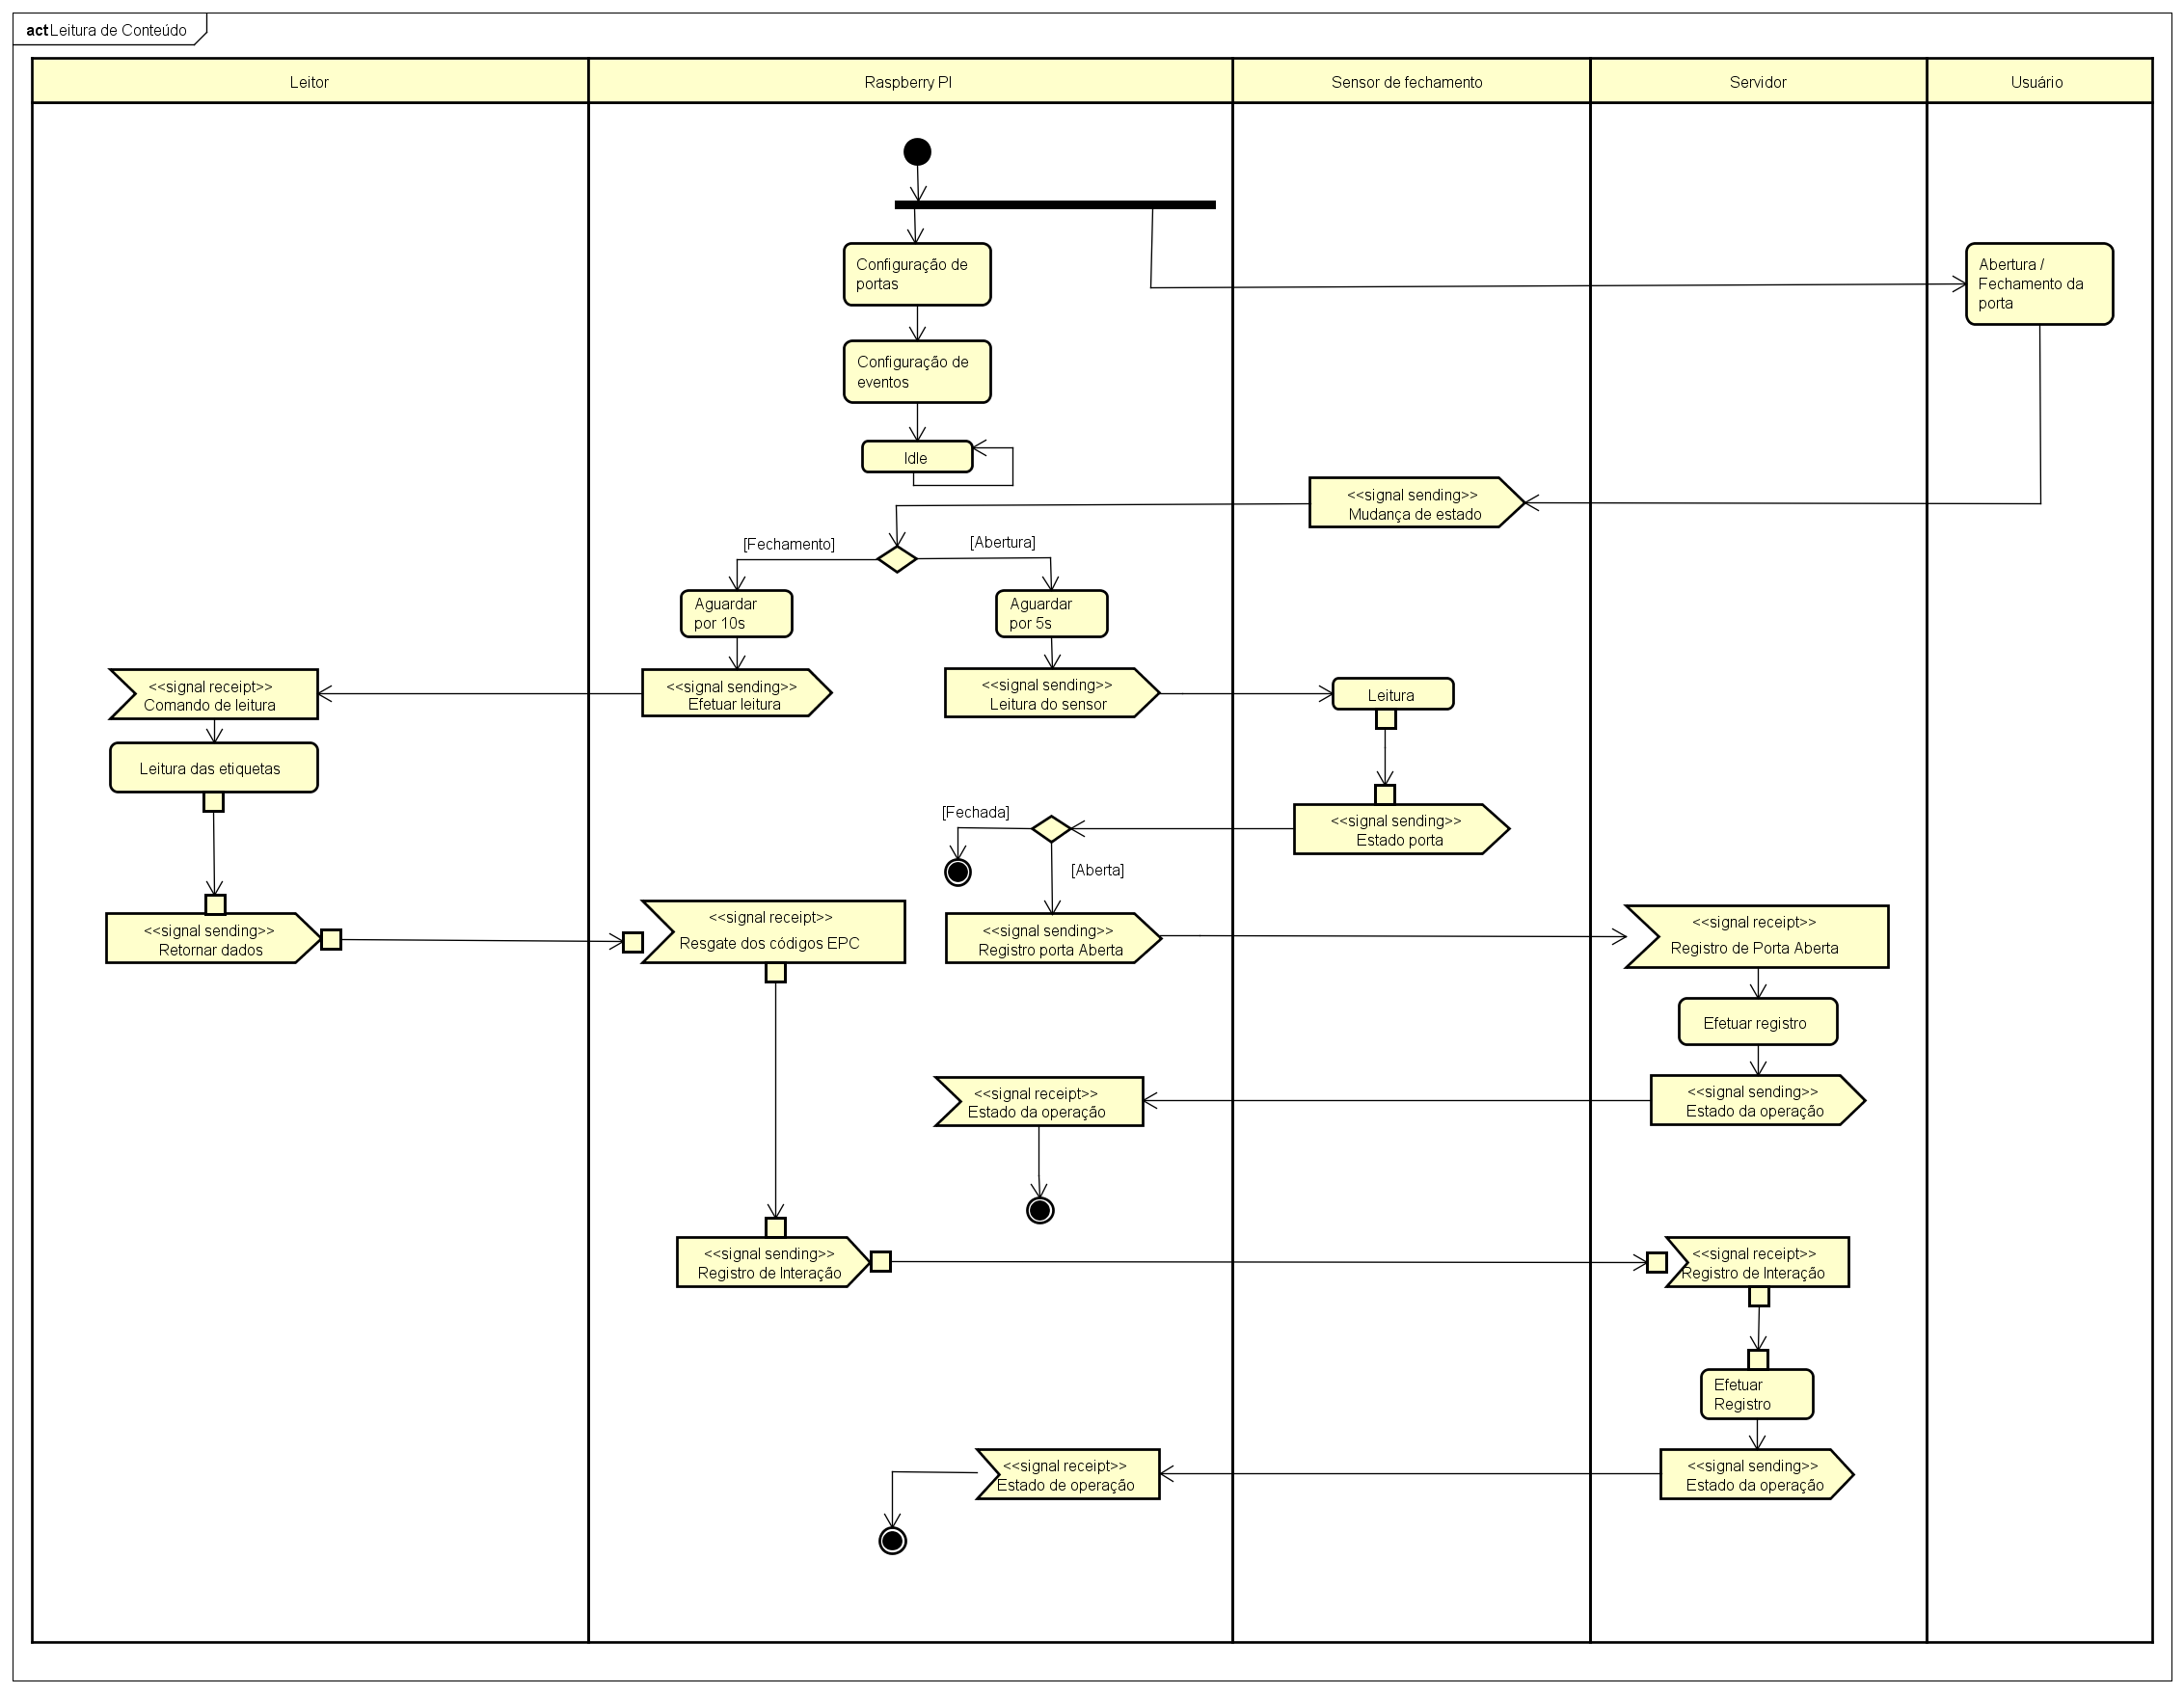
\includegraphics[height=0.9\textwidth, angle=90]{diagramas/diagr_leitura.png}
    
    \footnotesize{Fonte: Elaborado pelo Autor}
\end{figure}

%%%%%%%%%%%%%%%%%%%%%%%%%%%%%%%%%%%%%%%%%%%%%%%%%%%%%%%%%%%%%%%%%%%%%%%%%
\subsection{Listagem do Conteúdo da Geladeira}

Como  continuação do processo anterior, o processo de listagem de produtos disponibiliza na interface de usuário o conjunto de produtos disponíveis. A Figura \ref{fig:cap5_diagr_lista_prod} demonstra o fluxo de atividades para este processo.

O gatilho para tal ação é provido na interface de usuário e esta enviará uma requisição da lista de produtos referentes à uma geladeira específica. Ao receber a solicitação, o servidor realiza uma busca na base de interações pelo último registro gravado ao qual contém os códigos EPC lidos das etiquetas. Após isso, tendo o conjunto de códigos EPC, fará uma busca pelo produto correspondente a cada um. Assim, se terá uma lista de produtos e suas respectivas quantidades. Por fim, a lista de produtos, em formato JSON, é retornada à interface e apresentada ao usuário.

% Demonstrar fluxo de execução de listagem de produtos
\begin{figure}[htb]
    \caption{Fluxo para listagem de conteúdo da geladeira}
    \label{fig:cap5_diagr_lista_prod}
    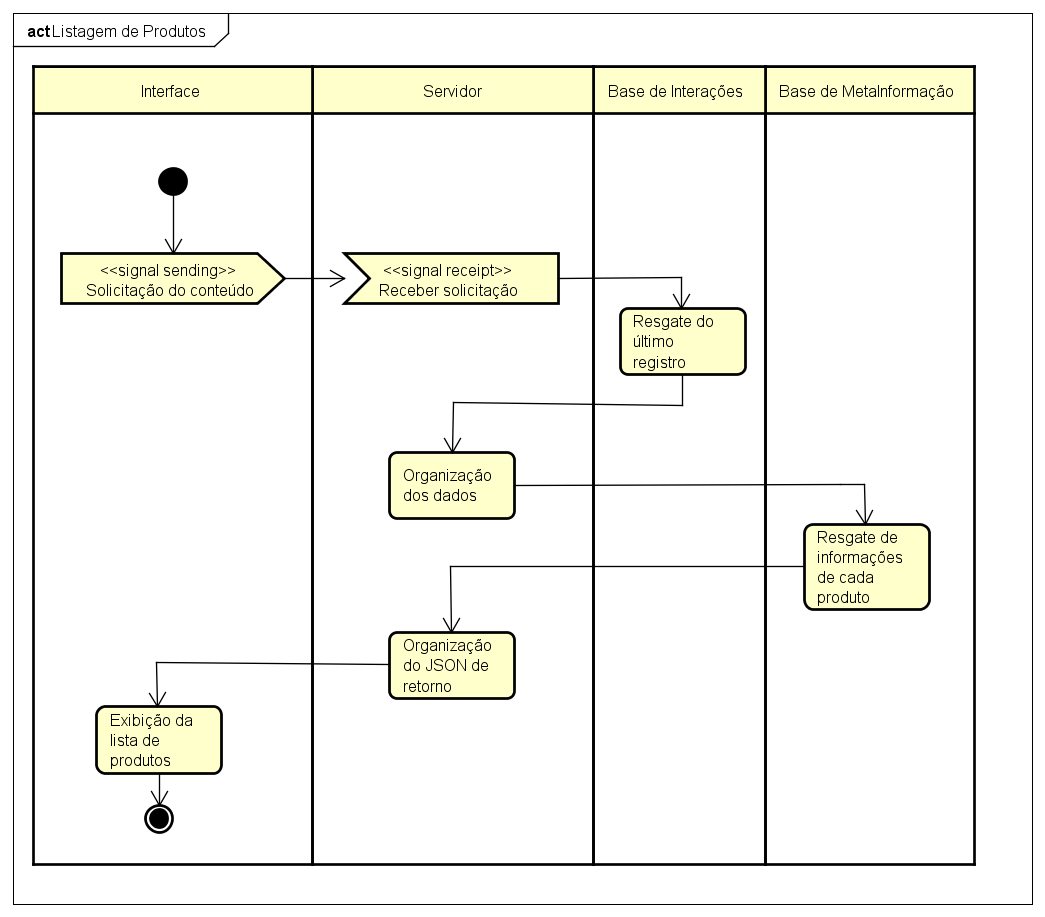
\includegraphics[width=\textwidth]{diagramas/diagr_lista_prod.png}
    
    \footnotesize{Fonte: Elaborado pelo Autor}
\end{figure}

\subsection{Recomendação de Produtos Novos} \label{ssec:geracao_rec_novo}

O processo de geração de recomendações, como já dito, é automaticamente inicializado pelo servidor, conforme Figura \ref{fig:cap5_diagr_geracao_rec}. Inicialmente, a matriz de frequência de interações de usuários com produtos é criada. Vale destacar, que um usuário está relacionado à uma geladeira. Em seguida, busca-se na base de interações todas as interações armazenadas. A partir das interações, na base de metainformação é efetuada a combinação entre códigos EPC e código de barras. A matriz de frequências é, então, preenchida com os dados obtidos no processo anterior.

Como parte do cálculo da correlação de Pearson, a média de interações de cada usuário deve ser calculada. Logo após, é computada a similaridade com a Equação \ref{eq:correlacao-pearson} entre os pares de usuários, indicados na Figura \ref{fig:cap5_diagr_geracao_rec} como $U1$ e $U2$.

Utilizando as similaridades calculadas inicia-se o processo de recomendação para cada usuário ($U1$) cadastrado no sistema. Inicialmente, o conjunto de similaridades do usuário $U1$ com os demais é ordenado em ordem decrescente, ou seja, do usuário com maior similaridade ao menor. Em seguida, para cada usuário $U2$ na lista de similaridades é realizada uma subtração de conjuntos de produtos aos quais $U2$ interagiu pelos itens que $U1$ interagiu. Assim, tem-se um conjunto de produtos que $U1$ não conhece e que poderão ser sugeridos como novas opções de compra. 

O processo citado é repetido até que todos os indivíduos na lista de usuários similares forneçam recomendações ou quando o número máximo de produtos recomendados for atingido. E quando uma das duas possibilidades ocorrer, o conjunto de recomendações será salvo na base de recomendações e o processo de recomendação se repetirá para o próximo usuário.

% Demonstrar fluxo de execução de geração de recomendação
\begin{figure}[H]
    \caption{Fluxo para recomendação de produtos novos} 
    \label{fig:cap5_diagr_geracao_rec}
    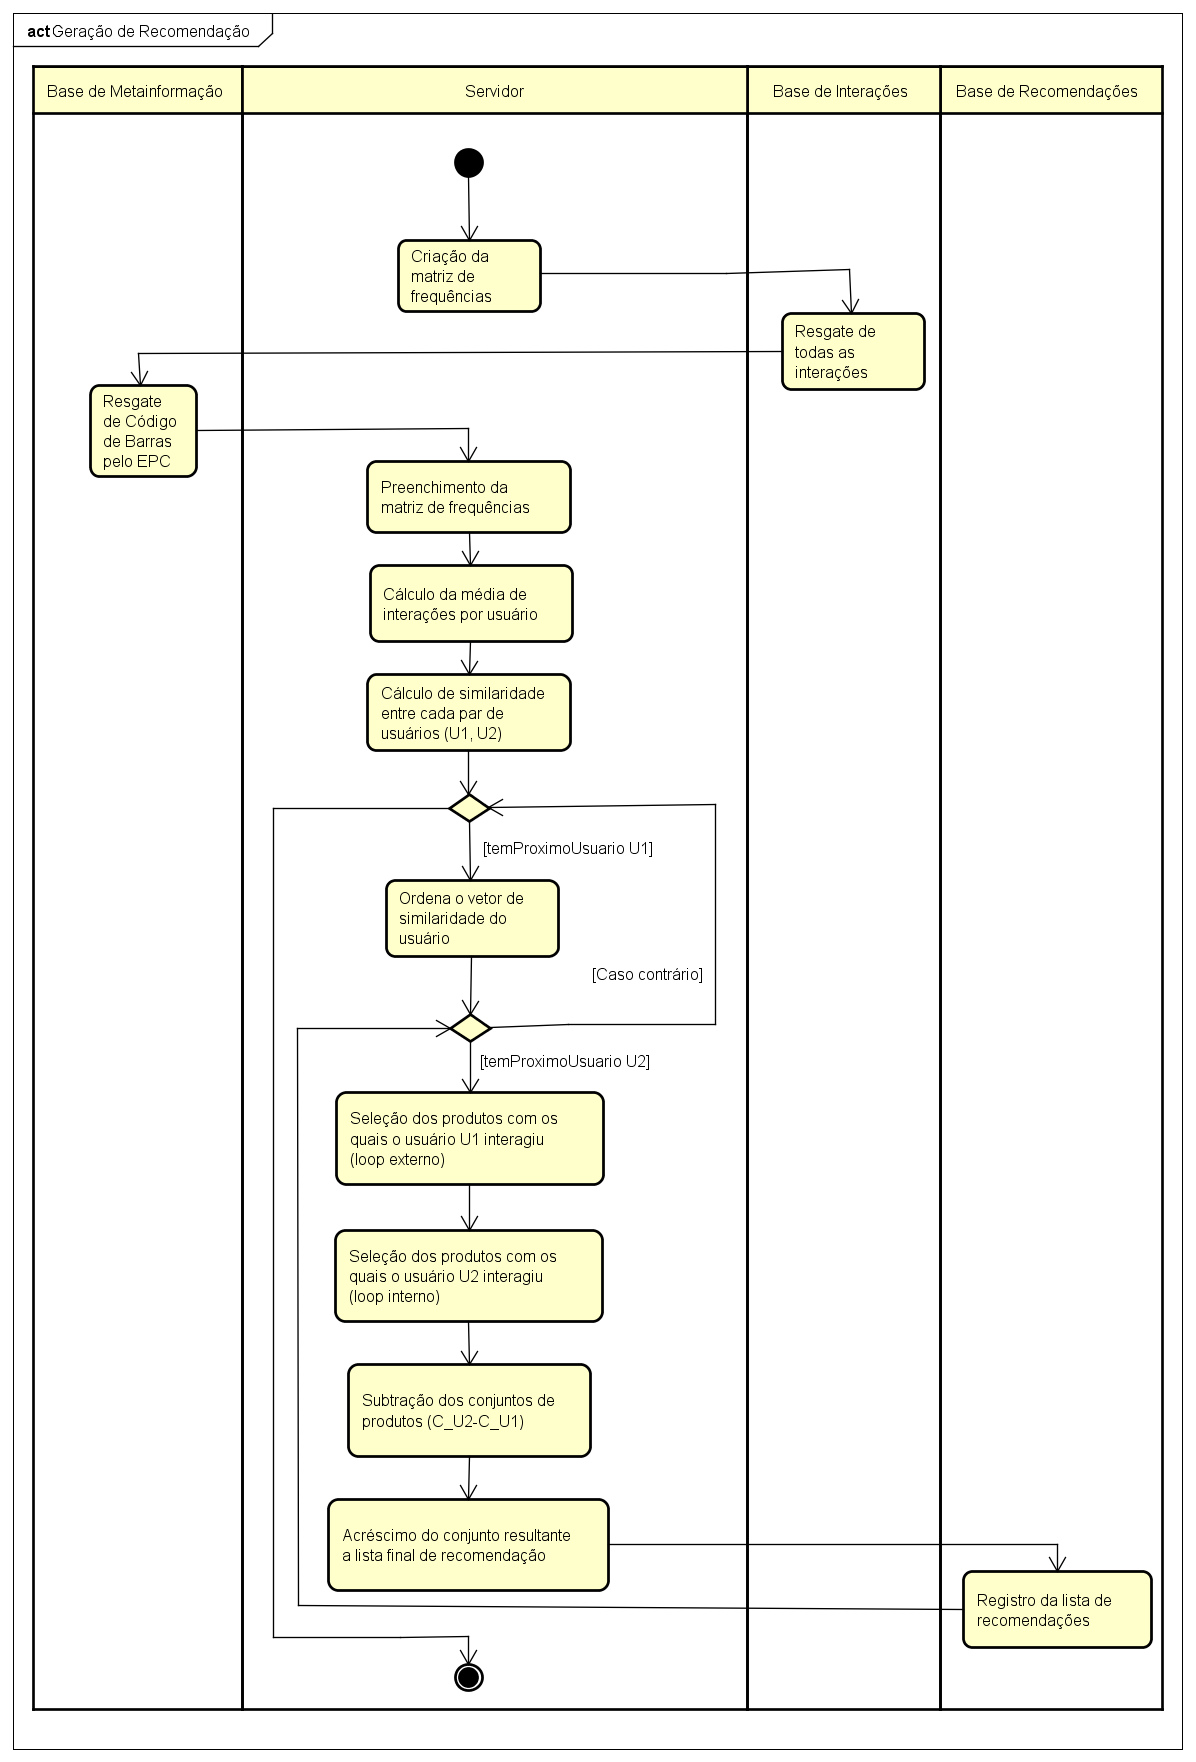
\includegraphics[width=\textwidth]{diagramas/diagr_geracao_rec.png}
    
    \footnotesize{Fonte: Elaborado pelo Autor}
\end{figure}

%%%%%%%%%%%%%%%%%%%%%%%%%%%%%%%%%%%%%%%%%%%%%%%%%%%%%%%%%%%%%%%%%%%%%%%%%
\subsection{Recomendação de Produtos Faltantes} \label{ssec:cap5_rec_prod_falt}

Da mesma forma que a seção anterior, o processo de recomendação é iniciado automaticamente pelo servidor, conforme Figura \ref{fig:cap5_rec_produto_faltante}. A partir disso, para que se recomende produtos é necessário ter as listas de produtos disponíveis atualmente e de produtos requisitados. Para tanto, inicialmente, a base de interações é consultada para o resgate da última interação, tendo esta a indicação dos itens mais recentes. A partir da lista de códigos EPC extraídos das interações é realizada uma consulta à base de metainformação para que sejam obtidos os dados dos produtos.

O próximo passo consiste na obtenção, na base de estruturas auxiliares, das informações de configuração do usuário, às quais indicam os produtos essenciais. A partir da extração dessas informações é efetuada uma comparação de quantidade entre produtos disponíveis e essenciais. Caso o produto essencial esteja disponível na quantidade necessária, nada acontece. No entanto, caso o produto esteja disponível e em quantidade insuficiente, este é inserido na lista de recomendações tendo como quantidade sugerida a diferença entre o valor necessário e o existente. Caso o produto necessário não exista, sugere-se a quantidade total indicada nas configurações.

A seguir, para o conjunto de produtos recomendados, é executada uma verificação no mercado sobre a disponibilidade dos mesmos conforme a quantidade especificada no passo anterior. Assim, caso o item esteja acessível, uma indicação positiva será retornada. Caso contrário, o serviço do mercado fará uma busca por um produto similar e retornará tal item como alternativa. Por fim, podem haver casos em que nenhum item similar exista. Assim, apenas uma indicação negativa é retornada.

Com o conjunto de produtos indicados pelo mercado como disponíveis para compra, a lista final de recomendações é criada e inserida na base de recomendações.

\begin{figure}[H]
    \caption{Fluxo para recomendação de produtos faltantes} 
    \label{fig:cap5_rec_produto_faltante}
    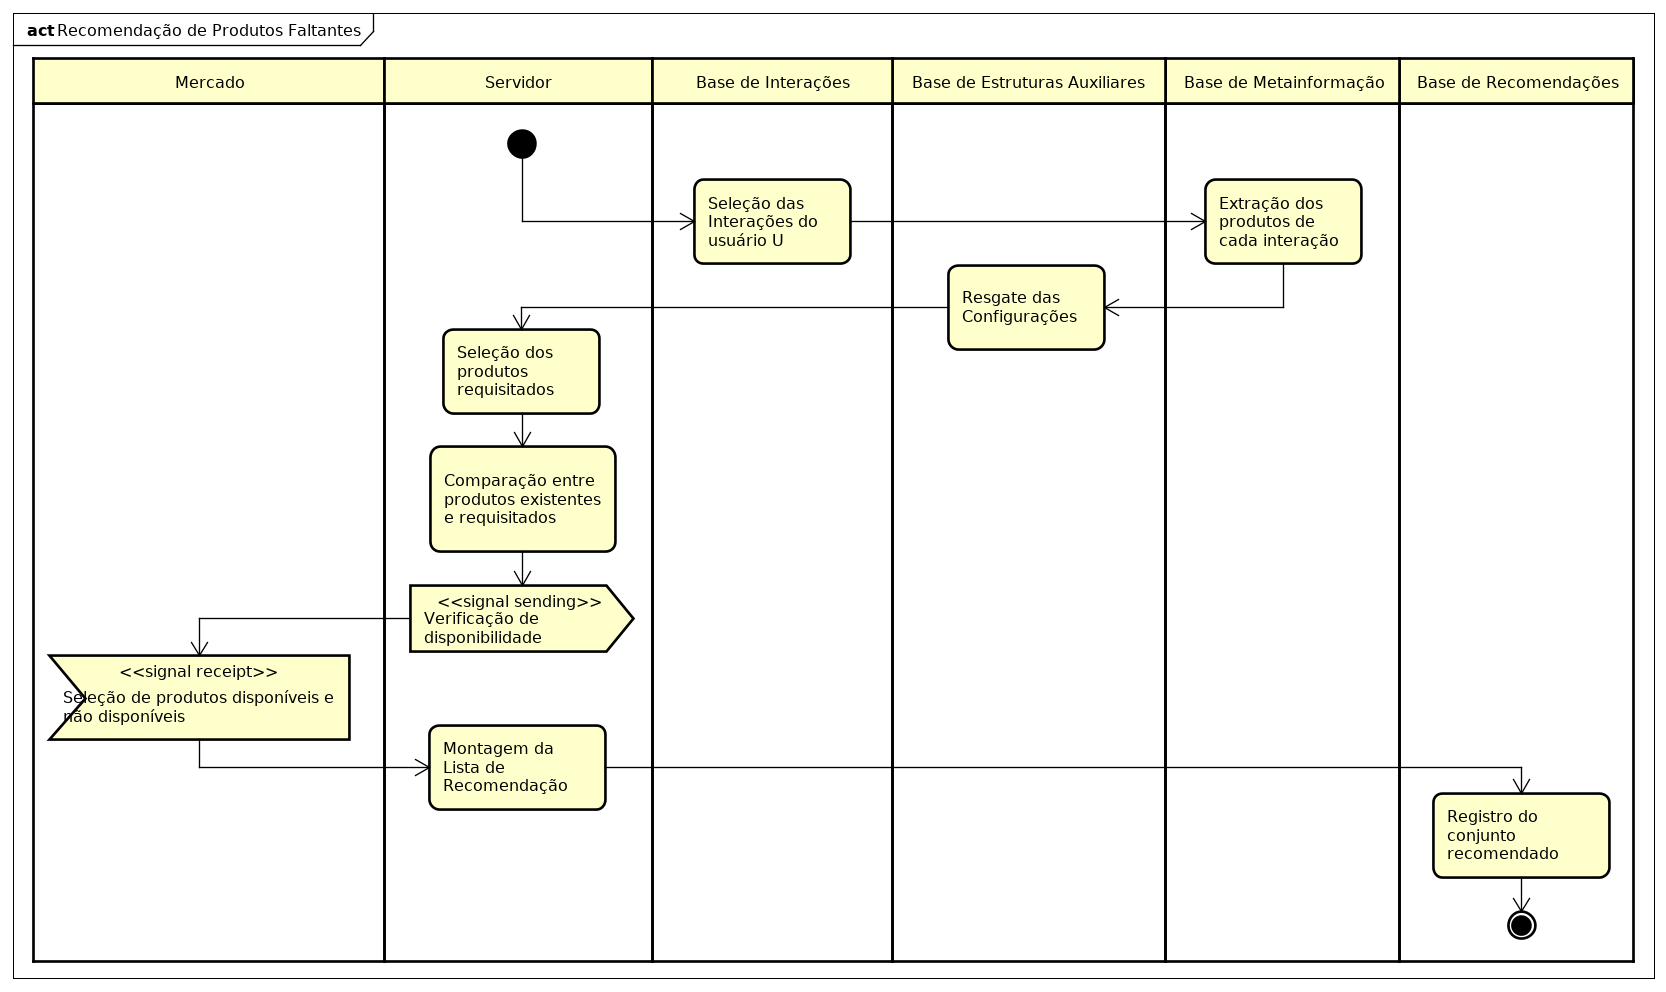
\includegraphics[width=\textwidth]{cap5_rec_produto_faltante}
    
    \footnotesize{Fonte: Elaborado pelo Autor}
\end{figure}

%%%%%%%%%%%%%%%%%%%%%%%%%%%%%%%%%%%%%%%%%%%%%%%%%%%%%%%%%%%%%%%%%%%%%%%%%
\subsection{Recomendação de Receitas por Conteúdo}

O processo de recomendação, conforme descrito na Seção \ref{sssec:proc_ger_rec}, decorre a partir da recomendação de receitas que contenham alguns dos produtos disponíveis na geladeira. 

O processo é iniciado automaticamente no servidor e o primeiro passo ocorre por meio na seleção da última interação, contendo os códigos EPC, na respectiva base de dados.

A partir dos códigos EPC, obtém-se o conjunto de produtos correspondentes a ele considerando a base de metainformação. Então, seleciona-se na base de metainformação as receitas que contenham pelo menos um dos produtos do conjunto. A partir do número de correspondências entre produtos da lista selecionada e da receita o conjunto de receitas é ordenado em ordem descendente, ou seja, receitas com maior número de correspondências primeiro. Por fim, o conjunto gerado é registrado na base de recomendações.

\begin{figure}[H]
    \caption{Fluxo para recomendação de receitas por conteúdo} 
    \label{fig:cap5_rec_receita_conteudo}
    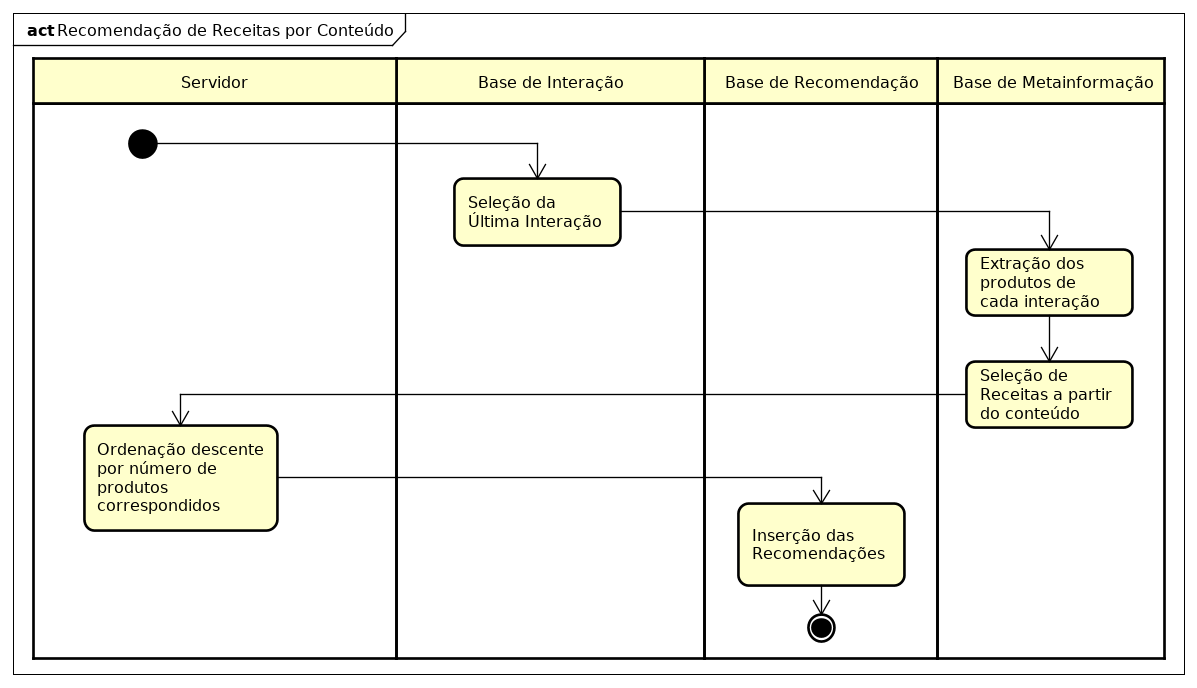
\includegraphics[width=\textwidth]{cap5_rec_receita_conteudo}
    
    \footnotesize{Fonte: Elaborado pelo Autor}
\end{figure}

%%%%%%%%%%%%%%%%%%%%%%%%%%%%%%%%%%%%%%%%%%%%%%%%%%%%%%%%%%%%%%%%%%%%%%%%%
\subsection{Recomendação de Receitas por Perfil}

A sugestão de receitas por perfil, conforme Figura \ref{fig:cap_diagr_receita_perfil}, considera os produtos com os quais o usuário mais interagiu durante a escolha de quais receitas recomendar. 

E, como nos demais processos, inicia-se no servidor automaticamente. 
O primeiro passo consiste na seleção de todas as interações do usuário na base de interações, seguida pela extração dos produtos de cada interação na base de metainformação. A partir disso, a matriz de frequências é criada e preenchida com base nos obtidos e da quantidade de vezes em que aparecem nas interações. O próximo passo, portanto, é a ordenação descendente através da frequência. Os produtos com maior frequência serão, então, utilizados como base na seleção de receitas. Nessa implementação, limitou-se em cinco (5) o número de produtos utilizados.

Com a lista de produtos, obtém-se o conjunto de receitas que contêm pelo menos um desses itens. O próximo passo consiste em ordenar a lista em disposição descendente a partir do número de produtos na receita correspondidos na lista de produtos.

Por fim, o conjunto de receitas sugeridas é registrado na base de recomendações.

\begin{figure}[H]
    \caption{Fluxo para recomendação de receitas por perfil} 
    \label{fig:cap_diagr_receita_perfil}
    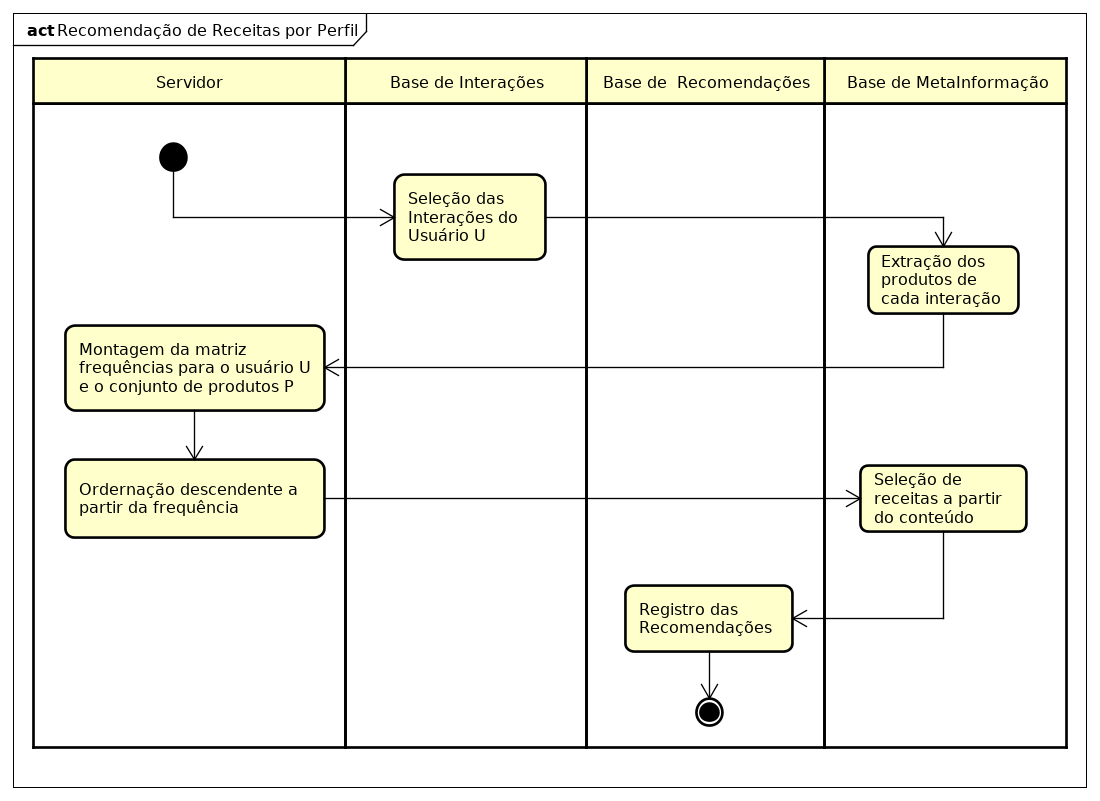
\includegraphics[width=\textwidth]{cap_diagr_receita_perfil}
    
    \footnotesize{Fonte: Elaborado pelo Autor}
\end{figure}

%%%%%%%%%%%%%%%%%%%%%%%%%%%%%%%%%%%%%%%%%%%%%%%%%%%%%%%%%%%%%%%%%%%%%%%%%
\subsection{Fluxo para Detecção e Registro de Porta Aberta}

Considerando-se, inicialmente, que a geladeira se encontra fechada. Em uma dado momento, o usuário abre-a e insere e/ou retira produtos, podendo, ao final, não fechar a porta. No momento da abertura, o sistema da geladeira detecta a ação e inicia um período de espera. Ao final desse tempo, um registro correspondente ao estado da porta é inserido na base de estruturas auxiliares.

Com relação à consulta de estado da porta, apesar de seu respectivo diagrama não ser apresentado neste trabalho, o fluxo é muito semelhante aos relacionados à consulta de listagem de produtos. Assim, quando a interface de usuário solicita o estado atual no servidor receberá o último registro realizado. A partir dele, caso indique estado aberto, uma notificação é emitida na interface.

\begin{figure}[H]
    \caption{Detecção de porta aberta}
    \label{fig:cap5_diagr_porta_aberta}
    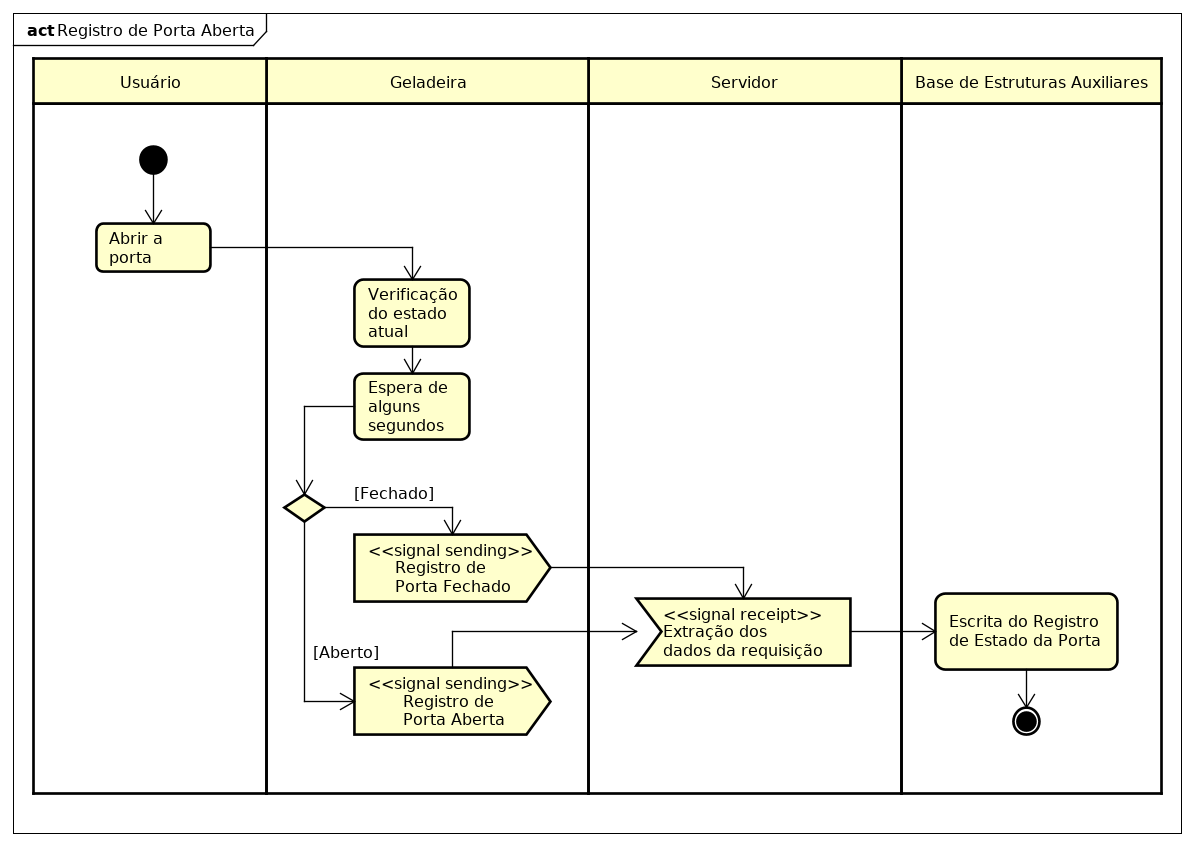
\includegraphics[width=\textwidth]{cap5_diagr_porta_aberta}
    
    \footnotesize{Fonte: Elaborado pelo Autor}
\end{figure}

\subsection{Listagem de Recomendações} \label{ssec:listagem_rec}

O processo de listagem de recomendações é disparado através da interface de usuário. Desse modo, a interface envia uma requisição ao servidor solicitando um conjunto de recomendações para um determinado usuário, conforme Figura \ref{fig:cap5_diagr_lista_rec}.  Ao receber a solicitação, o servidor faz uma busca na base de recomendações pelos produtos recomendados. Em seguida, os dados são organizados e o conjunto de recomendação é enviado à interface.

% Demonstrar fluxo de execução de listagem de recomendação
\begin{figure}[H]
    \caption{Fluxo para listagem de recomendações}
    \label{fig:cap5_diagr_lista_rec}
    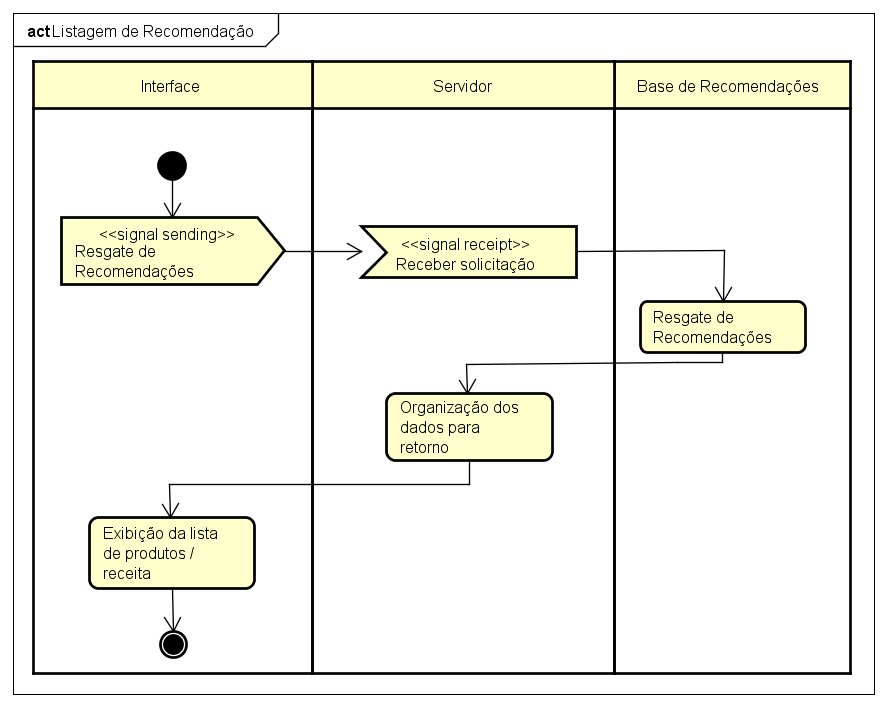
\includegraphics[width=\textwidth]{diagramas/diagr_list_rec.png}
    
    \footnotesize{Fonte: Elaborado pelo Autor}
\end{figure}

% Demonstrar fluxo de execução de listagem de produtos

\section{Cenário de Aplicação}

A avaliação do modelo dar-se-á a partir do ambiente ilustrado na Figura \ref{fig:cap5_ambiente-cenario}. O ambiente consiste na demonstração de uma sequência de ações, começando pela interação do usuário, com o objetivo de observar o comportamento e as funcionalidades do protótipo implementado.

\begin{figure}[htb]
    \caption{Ambiente do cenário}
    \label{fig:cap5_ambiente-cenario}
    \includegraphics[width=\textwidth]{figuras/cap5_cenario.png}
    
    \footnotesize{Fonte: Elaborado pelo Autor}
\end{figure}

Em relação, as bases de dados, essas foram preenchidas antes da avaliação do sistema. 
% Descrição dos dados de produtos
Primeiramente, para a base de metainformação foram alocadas informações de quarenta (40) produtos, extraídas de produtos originais a partir de um supermercado na cidade de Araranguá. Por outro lado, a informação referente à URL da imagem do produto foi obtida em \textit{websites} de supermercados.
%Excetua-se apenas o endereço URL da imagem de cada produto ao qual foi obtido \textit{websites} de supermercados. 
% Descrição de dados de receitas
Já em relação às receitas, utilizou-se dez (10) receitas obtidas a partir de sites de culinária. Tanto as informações de produtos quanto as receitas foram formatadas conforme a Seção \ref{sssec:metainfo}.

% Descrição da quantidade de usuários
Quanto à identificação das geladeiras e, por consequência, dos usuários, não criou-se uma base específica para eles, apenas atribuiu-se um identificador utilizado em cada registro específico a um determinado usuário. Como foram definidas dez (10) geladeiras, foram atribuídos os valores de um (1) a dez (10) para diferenciação de cada uma.

% Descrição da quantidade de interações por usuários.
Para cada geladeira, foram criadas, de maneira aleatória, interações, cada qual com um conjunto de códigos EPCs representando os produtos. Assim, definiu-se que o número de interações seria maior ou igual a cinco (5) e menor ou igual a 25. Além disso, para cada interação o número mínimo de itens registrados seria de três (3) e, no máximo, dez (10).

% Configurações de produtos
Em relação às configurações, descritas na Seção \ref{sssec:base_est-aux}, todas as geladeiras apresentaram parâmetros idênticos excetuando-se as listas de produtos essenciais e suas respectivas quantidades mínimas. Assim, tais produtos e suas respectivas quantidades foram definidos randomicamente para cada usuário.
%Assim, quais produtos e quais quantidades foram definidas randomicamente. 
Quanto à quantidade de produtos requisitados, estabeleceu-se o número de cinco (5) produtos e, em relação à quantidade, definiu-se um valor randômico entre um (1) e vinte (20).

% Quais os produtos que têm RFID que serão usados na geladeira
Como forma de teste do protótipo referente à estrutura física da geladeira, dois produtos receberam etiquetas com o respectivo código EPC, sendo eles, a ``Margarina com Sal Qualy\textsuperscript{\textregistered}\footnote{http://qualy.com.br/}'' e ``Creme de Leite Tirol\textsuperscript{\textregistered}\footnote{http://www.tirol.com.br/pt/}''.

%%%%%%%%%%%%%%%%%%%%%%%%%%%%%%%%%%%%%%%%%%%%%%%%%%%%%%%%%%%%%%%%%%%%%%%%%%%%%%%%%%%%%%%%%%%%%%%%%%%%%%%%%%%%%%%%%%%%%%%%%%%%%%%%%%%%%%%%%%%%%%%%%%%%%%%%%%%%%%%%%%%%%%%%%%%%%%%%%%%%%%%%%%%%%%%%%%%%%%%%%%%%%%%%%%%%%%%%%%%%%%%%%%%%%%%%%%%%%%%%%%%%%%%%%%%%%%%%%%%%%%%
\section{Avaliação do Protótipo}

Nessa seção é descrita a avaliação do protótipo criado. Para tanto, este será aplicados aos fluxos desenvolvidos na Seção \ref{sec:fluxos-de-execucao}. Assim, para cada fluxo comparar-se-á os resultados obtidos com os esperados.

%<<Descrever aqui uma introdução para esta seção>>

\subsection{Leitura do Conteúdo}
 Inicialmente a geladeira está vazia.
 Ao adicionar dois produtos, sendo eles, a ``Margarina com Sal Qualy\textsuperscript{\textregistered}'' e ``Creme de Leite Tirol\textsuperscript{\textregistered}'', respectivamente, depois de alguns minutos os seguintes códigos EPC são lidos.
 
\begin{itemize}[noitemsep,topsep=5pt]
     \item 8665580279609348107299713701
     \item 8665580277303506451141610373
 \end{itemize}
 
 Os dados são, então, enviados ao serviço de registro de interação e o registro é gravado na base de interações, conforme apresentado no Quadro \ref{fig:cap5_registro_interacao}. 
 
 %%%%%%%% JSON DO REGISTRO  %%%%%%%%
 \begin{quadro}[htb]
     \caption{Registro de interação dos produtos}
     \label{fig:cap5_registro_interacao}
     
     \frame{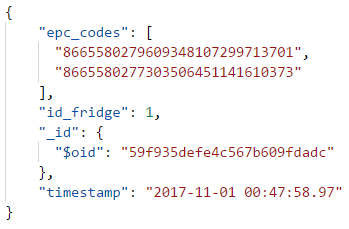
\includegraphics[width=0.5\textwidth]{cap5_registro_interacao}}
     
     \footnotesize{Fonte: Elaborado pelo Autor}
 \end{quadro}
 
\subsection{Listagem de Conteúdo da Geladeira}
 
Continuando o fluxo da seção anterior, ao tentar ler o conteúdo da geladeira logo após o fechamento da porta, a listagem da interface ainda se mantém vazia. Alguns segundos depois, a listagem é atualizada e o conteúdo exibido é mostrado na Figura \ref{fig:cap5_listagem_atual}.


 %%%%%%%%%%%%%%%%%%%%%   FIGURA DA LISTAGEM APÓS A INTERAÇÃO %%%%%%%%%%%%%%%%%%%%%%%%%%%%%%%%%%%
\begin{figure}[htb]
    \caption{Listagem de produtos na Interface}
    \label{fig:cap5_listagem_atual}
    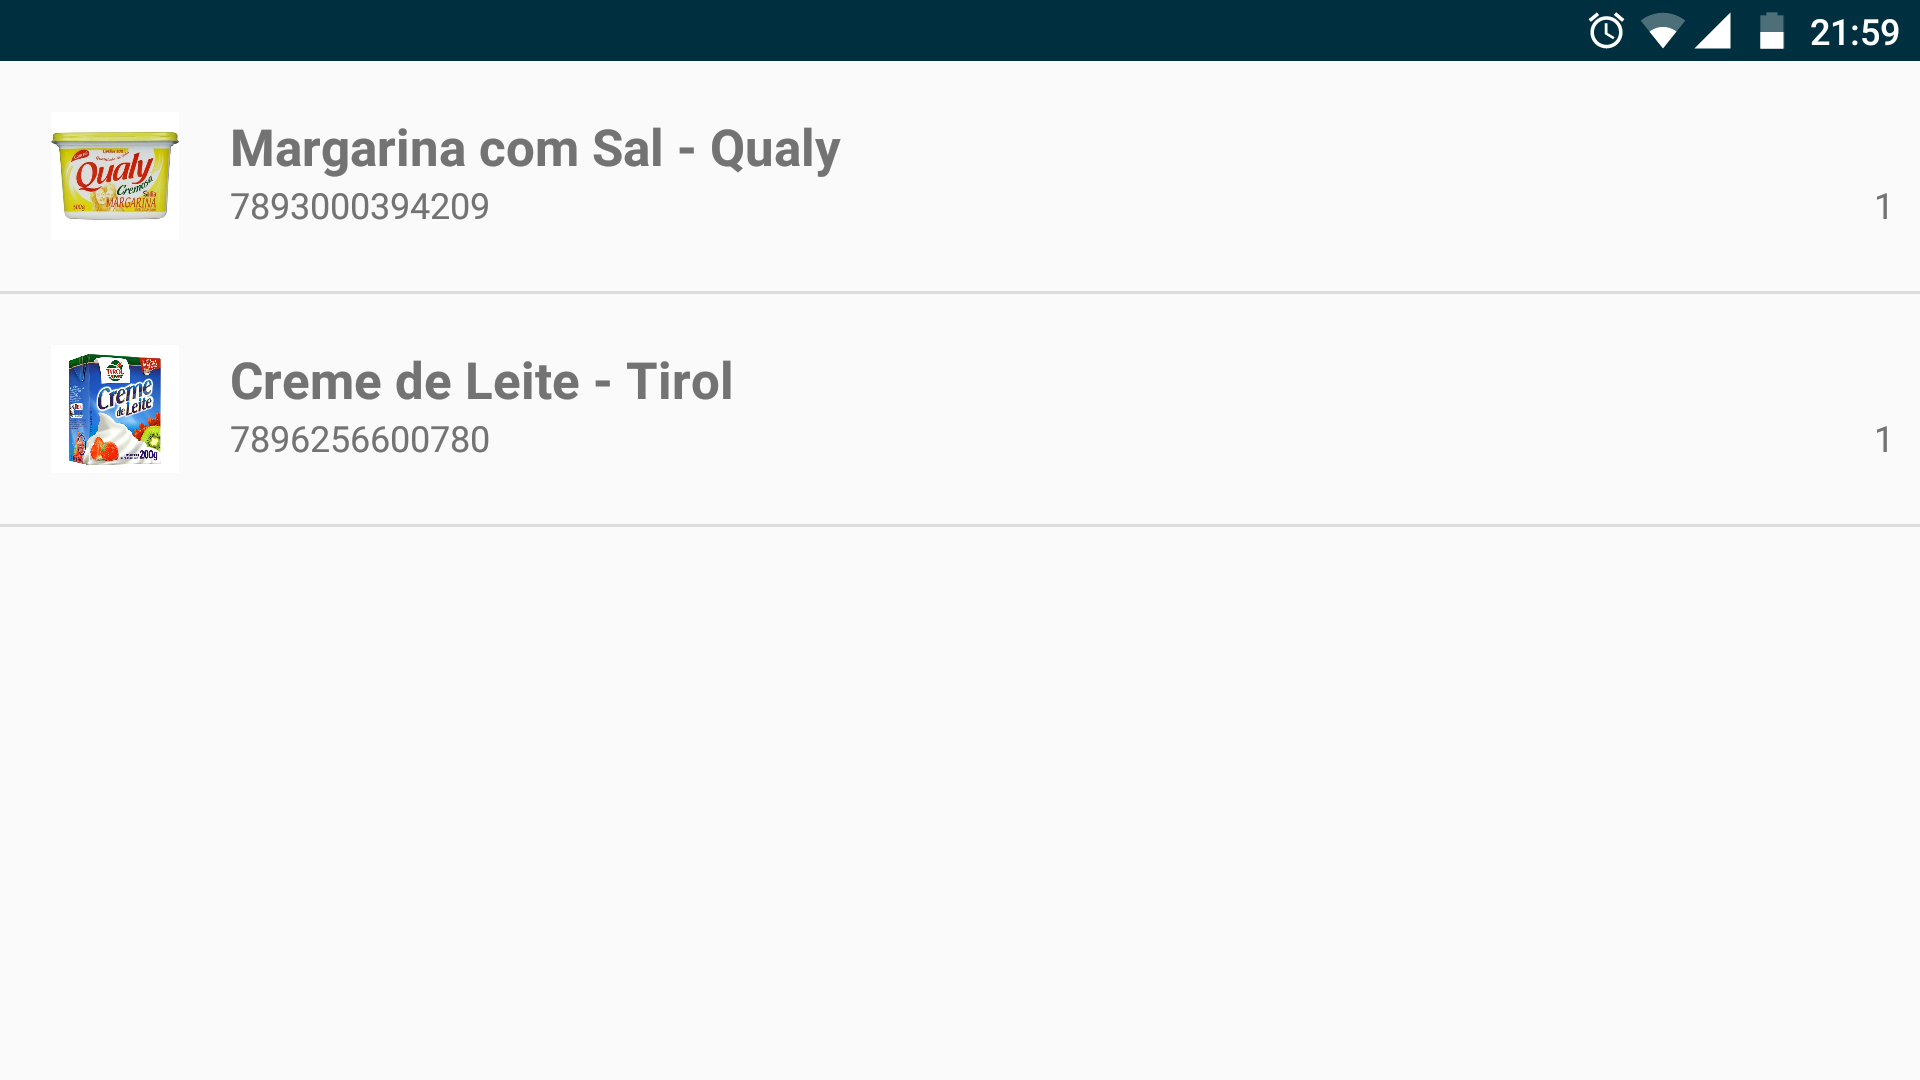
\includegraphics[width=0.8\textwidth]{cap5_listagem_atual}
    
    \footnotesize{Fonte: Elaborado pelo Autor}
\end{figure}
 
Dessa forma, afirma-se que a listagem de produtos produz resultados de acordo com o esperado, já que a lista é alterada após a interação. No entanto, o fator temporal entre a interação e a exibição é compreensível. Assim, o intervalo de tempo decorre do aguardo, na geladeira, até a realização da leitura. Isso é necessário para garantir que exista tempo hábil para coletar ou inserir todos os produtos que se deseja.


%%%%%%%%%%%%%%%%%%%%%%%%%%%%%%%%%%%%%%%%%%%%%%%%%%%%%%%%%%%%%%%%%%%%%%%%%%%%%%%%%%%%%%%%%%%%%%
\subsection{Recomendações de Produtos Novos}

Como exemplo, deseja-se gerar recomendações para o Usuário 1. Para tanto, seguiu-se o fluxo da Seção \ref{ssec:geracao_rec_novo}. Os passos foram executados até o cálculo de similaridade entre usuários sobre a matriz de frequências de interações e obteve-se o usuário mais semelhante. Tal indivíduo é identificado como Usuário 10 e o grau de similaridade entre este e o Usuário 1 foi de 0,15. A média de interações com produtos para o Usuário 1 foi de 2,05, já para o Usuário 10 foi de 2,12.

%inicia-se com a criação da matriz de frequências seguida pelo resgate das interações e, a partir dessas, dos códigos de barras e, por fim o preenchimento da matriz, conforme Figura \ref{fig:cap5_diagr_geracao_rec}.

Como forma de verificação, conforme Tabela \ref{tab:cap5_matriz_sim}, tem-se as linhas da matriz de frequência referentes aos usuários.


%%%%%%%%%%%%%%%%%%  MATRIZ  %%%%%%%%%%%%%%%%%%%%%%
\begin{table}[htb]
\caption{Matriz de frequências de interações}
\label{tab:cap5_matriz_sim}
%\begin{tabular}{C{0.72cm}c}
\toprule
\textbf{U1} \hspace{0.23cm} 0 2  2  6  2  3  6  0  2  4  2  5  2  1  1  2  1  8  5  6  5  1  2  3  3  5  5  3  1  0  0  0  0  0  0 \vspace{0.1cm} \midrule 
\textbf{U10} \hspace{0.02cm} 2  2  7  3  3  3  4  3  0  0  2  4  0  0  4  0  2  9  6  0  2  0  0  5  4  0  2  3  1  2  4  7  5  2  3 \vspace{0.1cm}  \bottomrule \vspace{0.1cm} 
%\end{tabular}

\footnotesize{Fonte: Elaborado pelo Autor}
\end{table}        

\newpage
Executando o cálculo da correlação de Pearson, descrita na Equação \ref{eq:correlacao-pearson}.

%%%%%%%%%%%%%%%%%%  EQUAÇÃO COM VALORES SUBSTITUÍDOS  %%%%%%%%%%%%%%%%%%%%%%%%%%%%%%
\begin{equation}
sim=\dfrac{\left[
\splitdfrac{
(0-2,05)(2-2,12)+
(2-2,05)(2-2,12)+
}
{\splitdfrac{
(2-2,05)(7-2,12)+
(6-2,05)(3-2,12)+
}{
(2-2,05)(3-2,12)+...}}\right]}
{
\left[
\splitdfrac{
\sqrt{\splitdfrac{(0-2,05)^2+
(2-2,05)^2+
(2-2,05)^2+
}{
(6-2,05)^2+
(2-2,05)^2+...}}
}{
\times\sqrt{\splitdfrac{(2-2,12)^2+
(2-2,12)^2+}{\splitdfrac{
(7-2,12)^2+
(3-2,12)^2+
}{
(3-2,12)^2+...}}}
}\right]
}
\nonumber
\end{equation}

\begin{equation}
sim = 0,15 \nonumber
\end{equation}

Assim, demonstra-se que o cálculo de similaridade está correto. Percebe-se que o número de produtos com os quais o Usuário 1 não apresentou nenhuma interação, ou seja, as posições na linha do usuário mencionado preenchidas com zero (0) é igual a oito (8). Assim, espera-se que pelos menos esses produtos sejam recomendados.

No entanto, um número maior de itens podem ser sugeridos. Isso ocorrerá quando a quantidade obtida de recomendações através do usuário com maior similaridade for insuficiente. Assim, recomendações de outros usuários com graus de semelhança menores serão consideradas.

Obteve-se, a partir da consulta à base de recomendações, a seguinte lista de itens:

\begin{itemize}[noitemsep,topsep=5pt]
%    \item 7892840800000 - Refrigerante Pepsi
    \item 789034630442 - Creme de Leite Parmalat
    \item 7894900093056 - Iogurte Danone
    \item 7896648699453 - Leite Integral Langaru
    \item 7894904326044 - Pizza Calabresa Seara
%    \item 7891991010481 - Cerveja Budweiser
    \item 7896256603422 - Leite Desnatado Tirol
    \item 7896256602050 - Iogurte de Morango Tirol
    \item 7891025101376 - Iogurte Danone
    \item 7896034680010 - Leite Condensado Parmalat
    \item 7891515490430 - Lasanha Calabresa Perdigão
\end{itemize}

 %%%%%%%%%%%%%%%%%%%%%   FIGURA DA LISTAGEM DE RECOMENDAÇÕES DE PRODUTOS NOVOS %%%%%%%%%%%%%%%%%%%%%%%%%%%%%%%%%%%

Os primeiros oito produtos da lista são aqueles que o Usuário 1 não interagiu, mas que o Usuário 10 o fez, na mesma sequência mostrada na Tabela \ref{tab:cap5_matriz_sim}. Já os demais itens foram sugeridos com base em outros usuários com menor similaridade. Vale ressaltar que o JSON gerado pelo sistema não foi inserido diretamente neste trabalho visto a extensão do mesmo.

\subsection{Recomendação de Produtos Faltantes}

Nesta seção, busca-se avaliar a recomendação da reposição de produtos aos quais o Usuário 2 julga serem essenciais. Para tanto, considera-se o fluxo de execução demonstrado na Seção \ref{ssec:cap5_rec_prod_falt} e o conjunto de produtos contidos atualmente e suas respectivas quantidades:

%%%%%%%%%%%%%%% Lista de um conjunto de produtos atuais %%%%%%%%%%%%%%%
\begin{itemize}[noitemsep,topsep=5pt]
    \item Mortadela Perdigão\textsuperscript{\textregistered} \footnote{http://www.perdigao.com.br/} 5 UN
    \item Pizza Calabresa Sadia\textsuperscript{\textregistered} \footnote{http://www.sadia.com.br/}, 4 UN
    \item Iogurte de Morango Activia\textsuperscript{\textregistered}\footnote{https://www.activiadanone.com.br/}, 5 UN
\end{itemize}

E o conjunto de produtos que o Usuário 2 estipulou que sempre devem estar à disposição:

%%%%%%%%%%%%%%% Lista de um conjunto de produtos essenciais %%%%%%%%%%%%%%%
\begin{itemize}[noitemsep,topsep=5pt]
    \item Mortadela, 8 UN
    \item Pizza Calabresa, 6 UN
    \item Iogurte de Morango, 5 UN
    \item Linguiça de Pernil, 15 UN
    \item Leite integral, 8 UN
\end{itemize}


Percebe-se que alguns produtos estão ausentes e, outros, em falta como, por exemplo, o produto Pizza está em quantidade insuficiente e o produto Leite está ausente. Assim, a recomendação deve conter tais produtos além dos outros não citados.

Seguindo o fluxo da Seção \ref{ssec:listagem_rec}, tem-se a listagem de sugestões na interface de usuário como é mostrado na Figura \ref{fig:cap5_rec_faltante}.

\begin{figure}[htb]
    \caption{Listagem de Recomendações por falta}
    \label{fig:cap5_rec_faltante}
    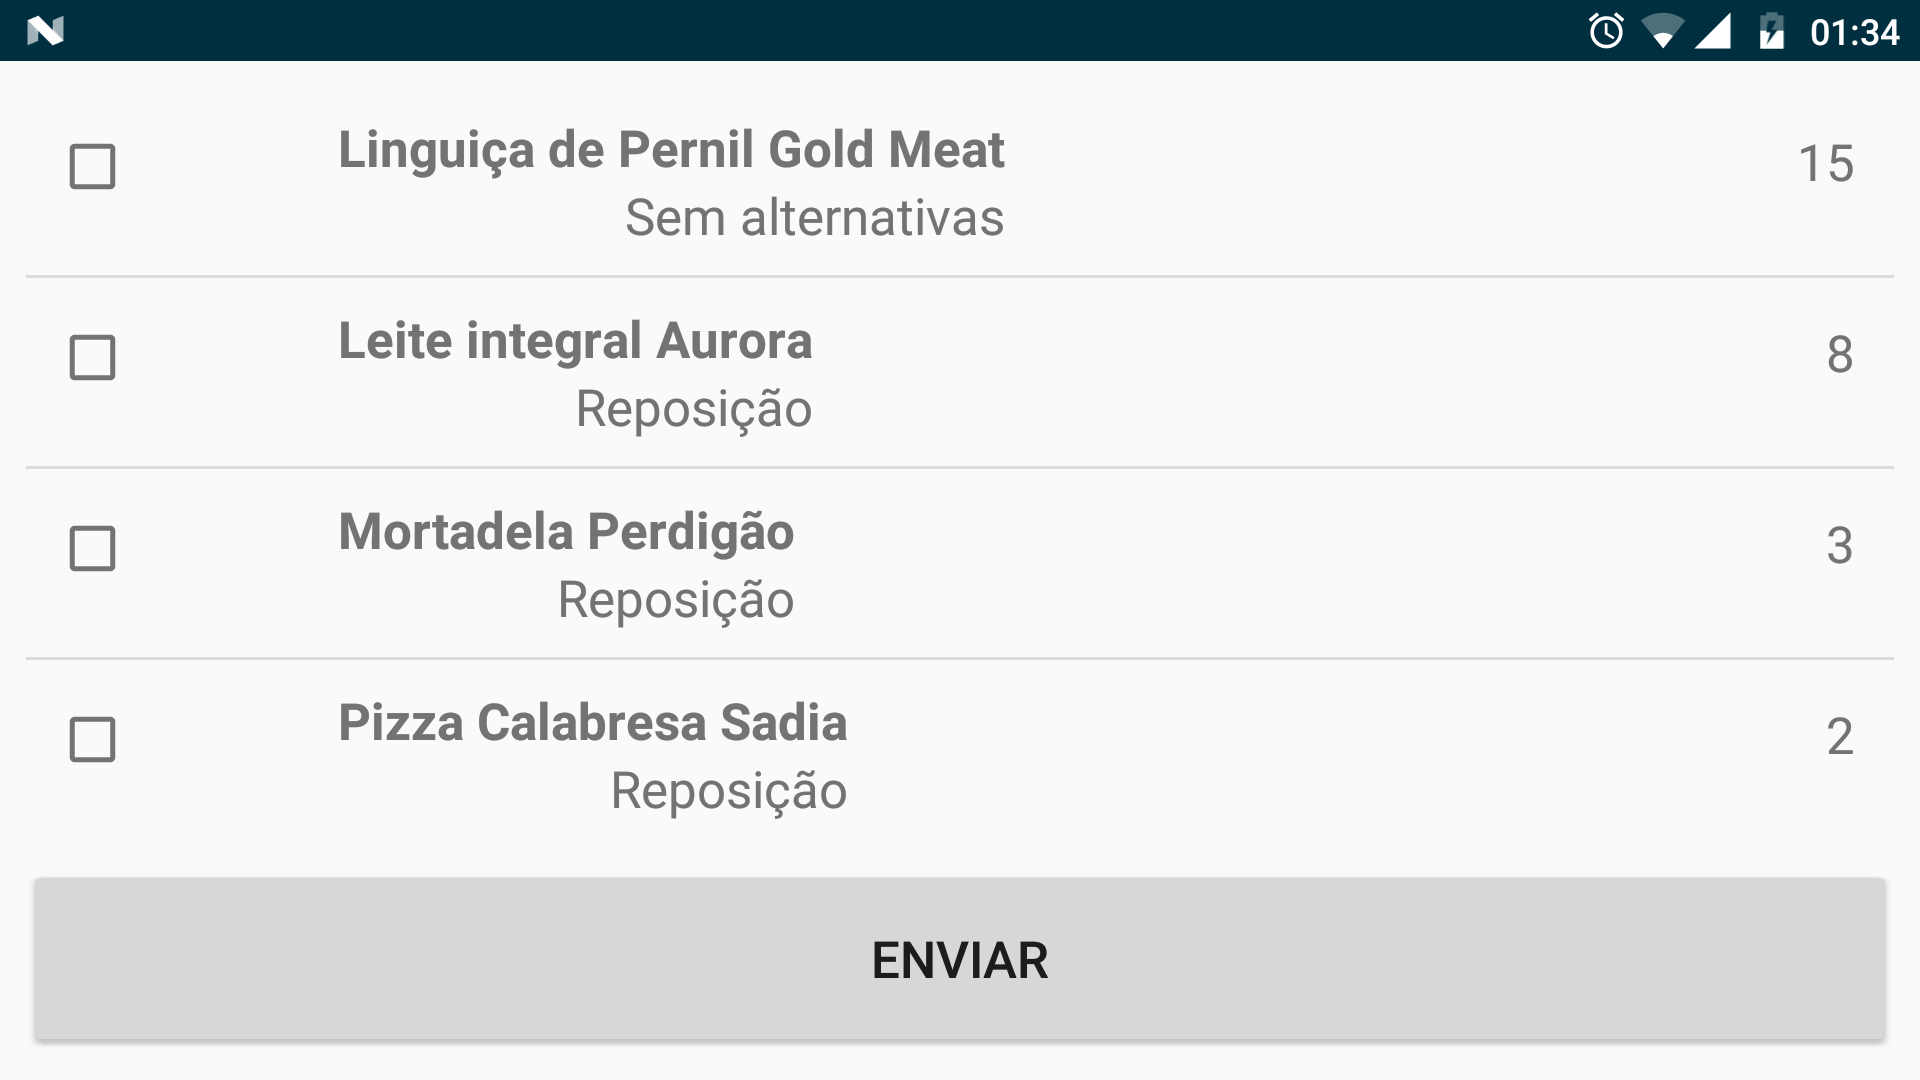
\includegraphics[width=0.8\textwidth]{cap5_rec_faltante}
    
    \footnotesize{Fonte: Elaborado pelo Autor}
\end{figure}

%%%%%%%%%%%%%%% Lista de um conjunto de produtos recomendados %%%%%%%%%%%%%%%

Pode-se verificar que há diferenciação entre os produtos, sendo de ``Reposição'' e ``Sem Alternativas''. A reposição trata da recolocação de produtos essenciais. O ``Sem alternativas'', indica que não foi possível encontrar no mercado, o produto esperado nem um similar a ele. Há, além disso, outras duas formas de recomendação de compras: ``Novo'', referente à recomendação de produtos novos, como descrito anteriormente, além de ``Similar'' que indica a reposição de produtos essenciais que não estavam disponíveis no mercado, mas que foram substituídos por produtos similares.

\subsection{Recomendação de Receitas a partir de Conteúdo}

A recomendação de receitas por conteúdo, como descrito na seção respectiva no Capítulo 4, busca disponibilizar um conjunto de receitas ao usuário de acordo com os itens que este possui em sua geladeira. 

Considera-se que, inicialmente, os seguintes produtos estejam disponíveis com suas respectivas quantidades:

\begin{itemize}[noitemsep,topsep=5pt]
    \item Leite Integral, com 2 UN
    \item Leite Condensado Parmalat\textsuperscript{\textregistered}\footnote{http://www.parmalat.com.br/}, com 3 UN 
    \item Queijo Mussarela Sadia\textsuperscript{\textregistered}, com 5 UN.
\end{itemize}

O processo de recomendação avaliará os produtos do ponto de vista de suas características, ou seja, terá um enfoque nos tipos de produtos e não em produtos de determinadas marcas.

O processo de recomendação analisa quais receitas satisfazem o requisito especificado e retornará um conjunto de itens como sugestão.

Os itens sugeridos como recomendações são mostrados na Figura \ref{fig:cap5_rec_recipe_content}.

%%%%%%%%%%%%%%%%%%    FIGURA X (Lista de receitas de recomendação)    %%%%%%%%%%%%%%%%%%%%%%%%%%%%%
\begin{figure}[htb]
\caption{Resultado da recomendação de receitas}
\label{fig:cap5_rec_recipe_content}
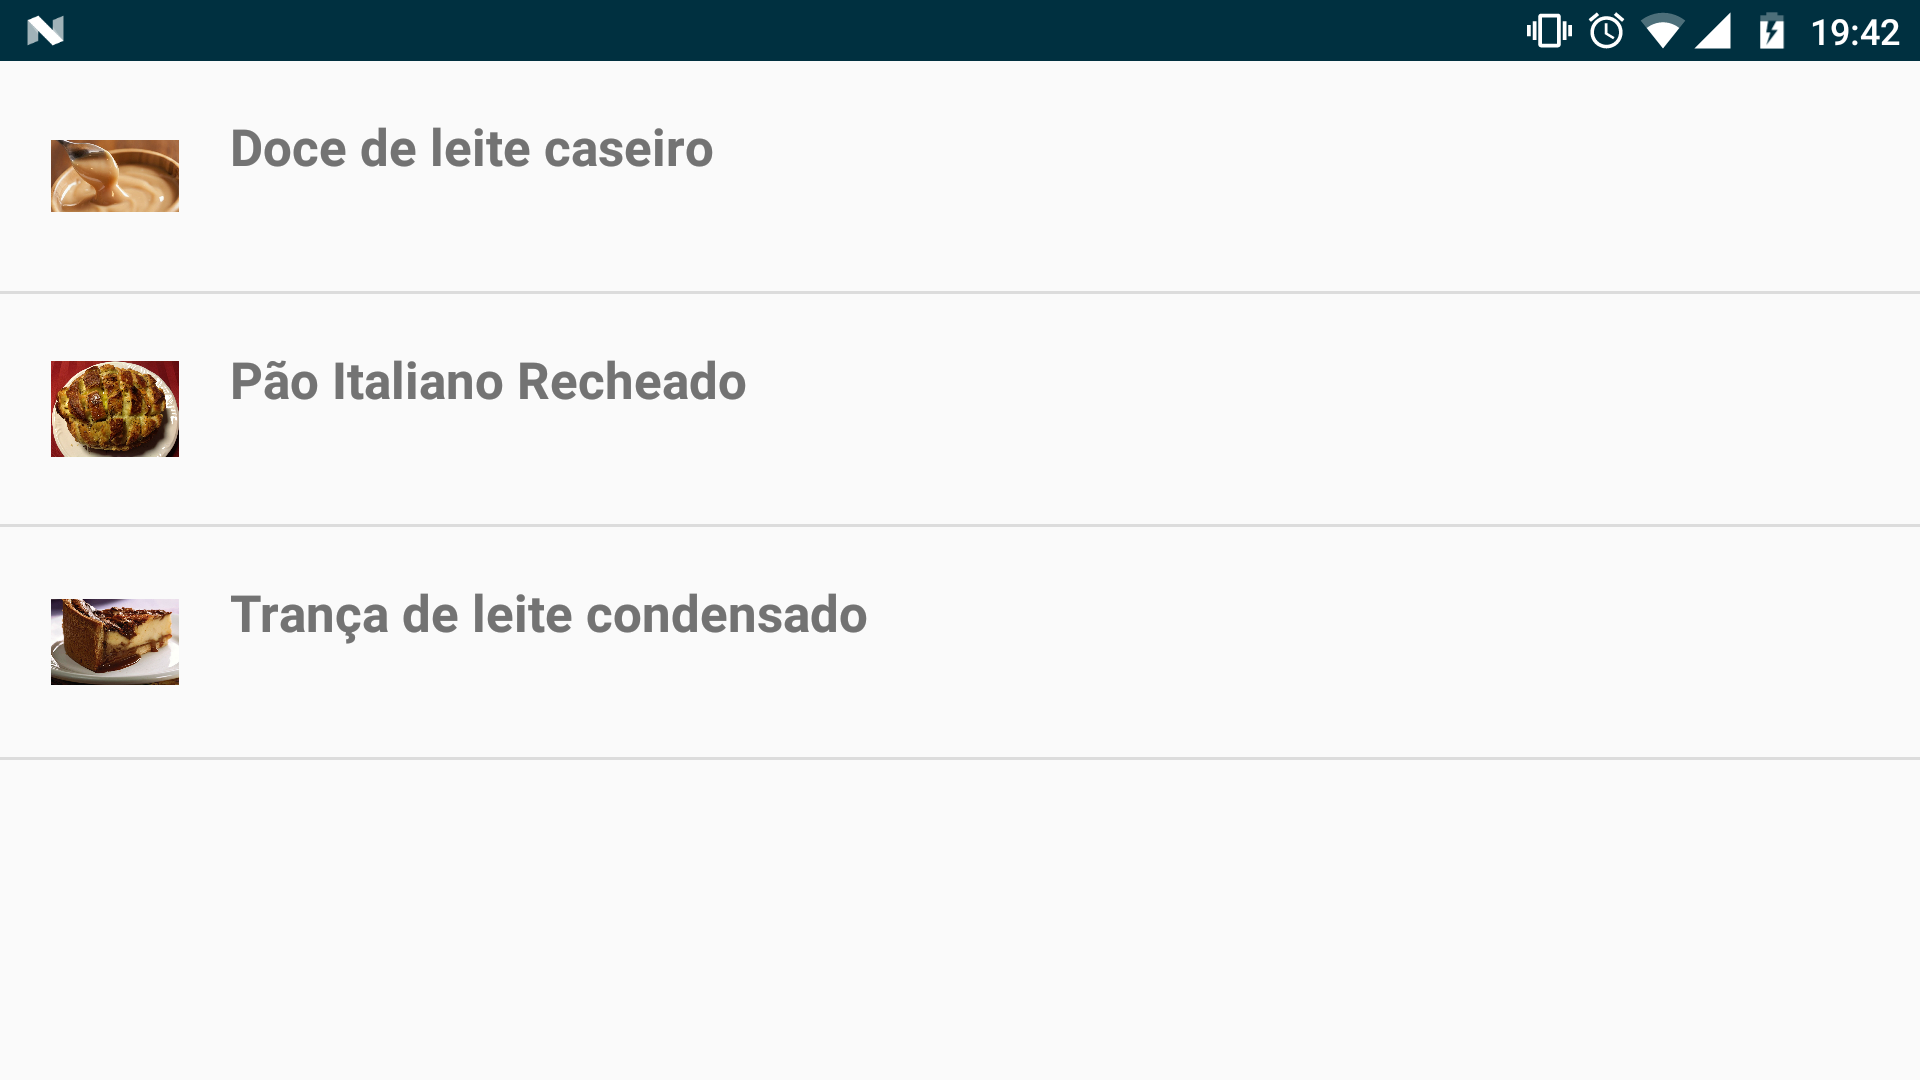
\includegraphics[width=0.8\textwidth]{cap5_rec_recipe_content}

\footnotesize{Fonte: Elaborado pelo Autor}
\end{figure}

Como resultado da recomendação, tem-se três receitas sugeridas dentre as cinco utilizadas nesse cenário, ou seja, duas receitas não incluíam nenhum dos produtos contidos na geladeira. A primeira receita na lista conta com o Leite, a segunda com o Queijo Mussarela e a terceira com Leite e Leite Condensado.

\subsection{Recomendação de Receitas por Perfil}

Como descrito na Seção \ref{sssec:proc_ger_rec}, a sugestão de receitas por perfil buscará receitas que contenham alguns dos itens com os quais o usuário mais interagiu. Para tanto, uma matriz de frequência de interações é elaborada. Com base nas frequências de interações do usuário em questão, uma lista é criada a partir das classes de produto.

Considerando que o total de produtos para geração de recomendação foi limitado em cinco (5) tem-se os seguintes produtos:

\begin{itemize}[noitemsep,topsep=5pt]
    \item Margarina com Sal Qualy, com 9 interações
    \item Refrigerante de Guaraná Fanta, com 9 interações
    \item Linguiça de Pernil Gold Meat, com 8 interações
    \item Iogurte Danone, com 7 interações
    \item Queijo Mussarela Sulfrios, com 7 interações
\end{itemize}

Com base neste conjunto, o processo de recomendação realiza uma busca na base de interações pela receitas que possuem tais categorias de produtos. A partir disso, o conjunto de receitas da Figura \ref{fig:cap5_rec_recipe_profile} foi sugerido.


%%%%%%%%%%%%%%%%%%%%%% FIGURA RECEITA SUGERIDA %%%%%%%%%%%%%%%%%%%%

\begin{figure}[htb]
    \caption{Lista de Receitas Sugeridas por Perfil}  
    \label{fig:cap5_rec_recipe_profile}
    
\includegraphics[width=0.8\textwidth]{cap5_rec_recipe_profile}
   
    \footnotesize{Fonte: Elaborado pelo Autor}
\end{figure}

Apesar de apenas uma receita ter sido sugerida, devido ao total de receitas muito reduzido do cenário, é possível validar a recomendação, já que esta conta com o produto Queijo Mussarela.

\subsection{Alerta de Porta Aberta}

%% OBJETIVO
Os alertas enviados aos usuários que esquecem a porta da geladeira aberta, ou não a fecham corretamente, é importante para evitar gastos desnecessários com energia e, possivelmente, com alimentos estragados. Como descrito na Seção \ref{ssec:c5_camada_servicos}, o processo de verificação de porta aberta, dispara um registro no servidor. Para o exemplo, considera-se que inicialmente a porta estava fechada e, em um dado momento, foi deixada aberta.

Após alguns segundos o registro do Quadro \ref{fig:cap5_open_door_reg} foi efetuado na base de estruturas auxiliares, informando a situação.


%%%%%%%%%%%%%%%%% REGISTRO DE PORTA ABERTA  %%%%%%%%%%%%%%%
\begin{quadro}[H]
    \caption{Registro de porta aberta}
    \label{fig:cap5_open_door_reg}
    \frame{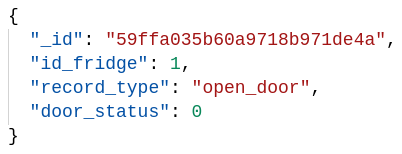
\includegraphics[width=0.5\textwidth]{cap5_open_door_reg}}
    
    \footnotesize{Fonte: Elaborado pelo Autor}
\end{quadro}

Algum tempo depois, a interface de usuário realiza uma requisição ao serviço de estado de porta. Neste caso, a aplicação da interface verificou que o estado era aberto e notificou ao usuário, conforme a Figura \ref{fig:cap5_open_door_alert}.


%%%%%%%%%%%%%%% IMG NOTIFICAÇÃO DE PORTA ABERTA  %%%%%%%%%%%%
\begin{figure}[H]
    \caption{Alerta de porta aberta}
    \label{fig:cap5_open_door_alert}
    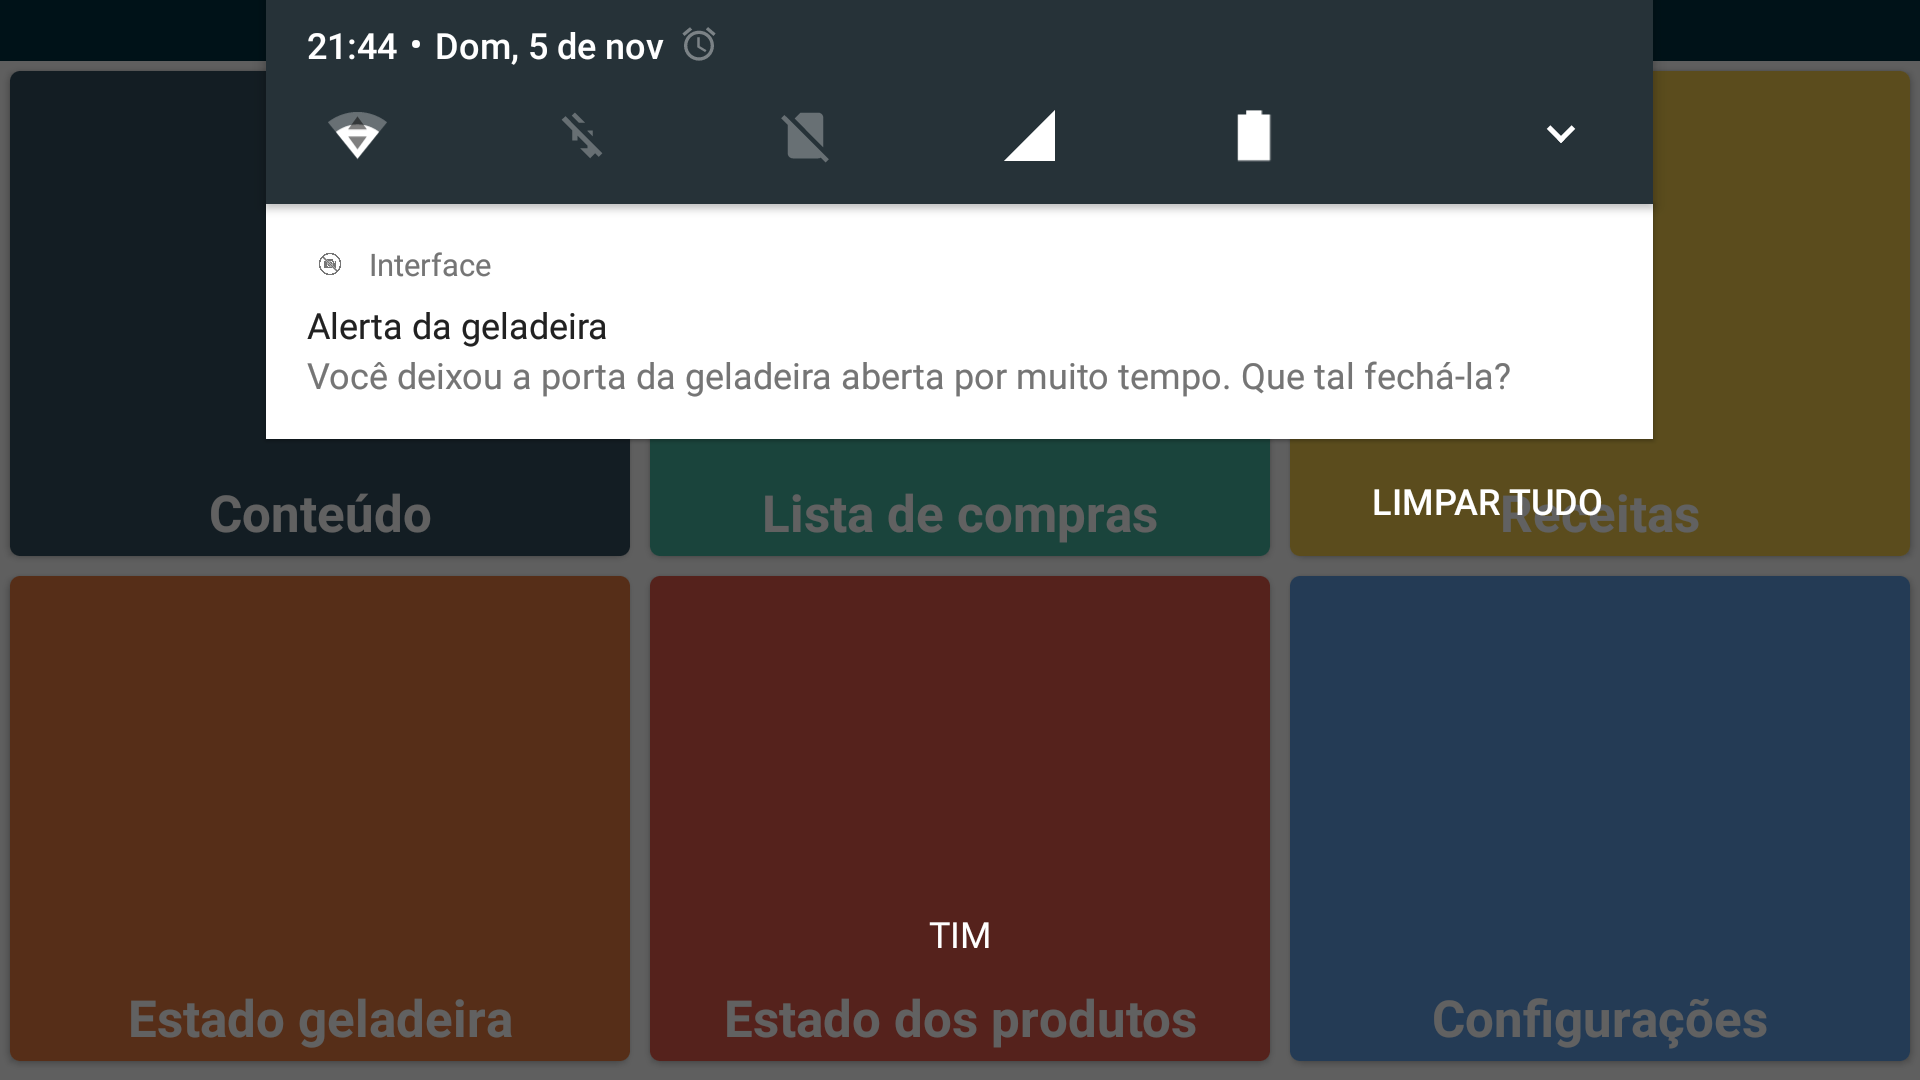
\includegraphics[width=\textwidth]{cap5_open_door_alert}
    
    \footnotesize{Fonte: Elaborado pelo Autor}
\end{figure}




